\documentclass[11pt,a4paper,british]{article}
\usepackage[latin1]{inputenc}
\usepackage[T1]{fontenc}
\usepackage{babel,url,graphicx}
\usepackage{listings, amsmath, amsfonts}
\title{Problem X}

\date{}


\begin{document}
\maketitle

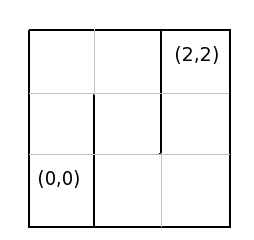
\includegraphics{hedge.png}

%\chapter*{Hedges}
\begin{center}
\Huge{Hedges}
\end{center}


So you find yourself trapped in the (0,0) square of a rectangular X$\times$Y hedge maze that is divided into unit squares.  You want to get to the exit which is in (X-1, Y-1).  Being a bit excentric, you will always increase exactly one of your coordinates by 1 at each step, minimizing the tootal number of steps.  This makes things a bit difficult, but luckily, you also have a team of self sacrificing heroes with you, so whenever you encounter a wall, you may leave one hero behind to help all the others climb over.

Now, what you would like to know is exactly how many of you can reach the exit this way.

\subsection*{Input}
The first line of input contains a single integer T, denoting the number of test cases.  Then for each test case there will be a line containing 3 integers, X, Y and M, denoting dimensions of the maze, and the number of heroes (including you).   The following X lines containins Y-1 numbers that are all 0 or 1.  There is a hedge between square (i,j) and (i,j+1) if and only if the j'th number on the i'th line is 1.  Then follows X-1 lines with Y numbers on each line, telling that there is a hedge between (i,j) and (i+1, j) if and only if the j'th number on the i'th line is 1.


\paragraph{Constraints}\ \\
$1\leq T \leq 100$\ \\
$2\leq X,Y \leq 300$\ \\
$2\leq M \leq 10^9$\ \\


\subsection*{Output}

For each test case, output one number on a single line, the maximal number of heroes that may reach the goal.

\paragraph{Sample input}\ \\
2\\3 3 4\\
1 0\\
1 1\\
0 1\\
0 0 0\\
0 0 0\\
3 2 2\\
1 \\
1\\
1 \\
1 1 \\
1 1 \\
\paragraph{Sample output}\ \\
3\\0\\
 


\end{document}
